\begin{minipage}{0.75\linewidth}
\begin{figure}[h]
    \centering
    \begin{adjustbox}{max width=1.0\linewidth, keepaspectratio}
        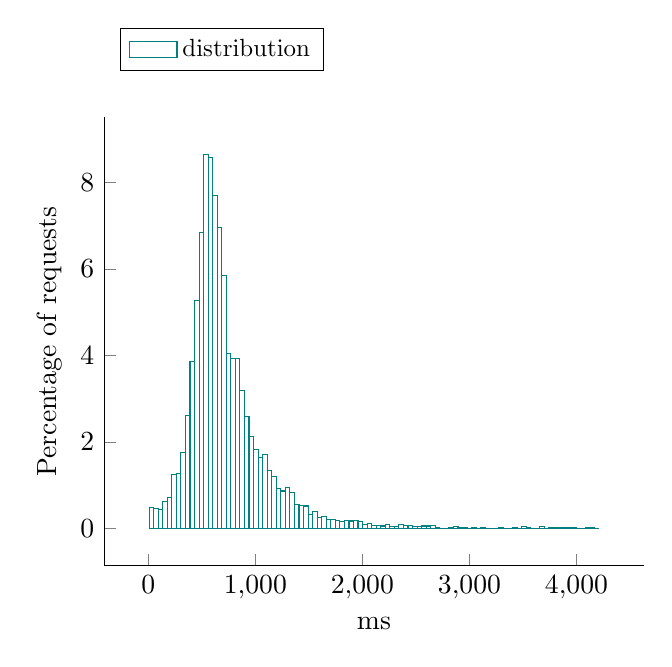
\begin{tikzpicture}
            \begin{axis}[ylabel = Percentage of requests, 
xlabel = ms, 
legend style = {nodes={scale=0.9, transform shape}, at={(0.03,1.2)}, anchor=north west, draw=black, fill=white, align=left, legend columns=3},
area style, mark size = 0pt,
 cycle list name = exotic,
  axis lines* = left]
		\addplot +[ybar interval] coordinates {
			 (7, 0.483549)
			 (49.44, 0.462525)
			 (91.88, 0.430989)
			 (134.32, 0.609692)
			 (176.76, 0.714811)
			 (219.2, 1.24041)
			 (261.64, 1.26143)
			 (304.08, 1.75549)
			 (346.52, 2.60696)
			 (388.96, 3.85788)
			 (431.4, 5.26648)
			 (473.84, 6.84327)
			 (516.28, 8.64081)
			 (558.72, 8.57774)
			 (601.16, 7.69473)
			 (643.6, 6.9589)
			 (686.04, 5.84463)
			 (728.48, 4.04709)
			 (770.92, 3.93146)
			 (813.36, 3.93146)
			 (855.8, 3.18512)
			 (898.24, 2.58594)
			 (940.68, 2.12341)
			 (983.12, 1.82908)
			 (1025.56, 1.63986)
			 (1068, 1.70293)
			 (1110.44, 1.33502)
			 (1152.88, 1.18785)
			 (1195.32, 0.92505)
			 (1237.76, 0.861978)
			 (1280.2, 0.946074)
			 (1322.64, 0.830443)
			 (1365.08, 0.54662)
			 (1407.52, 0.536108)
			 (1449.96, 0.515085)
			 (1492.4, 0.32587)
			 (1534.84, 0.388941)
			 (1577.28, 0.252286)
			 (1619.72, 0.262798)
			 (1662.16, 0.210239)
			 (1704.6, 0.199727)
			 (1747.04, 0.178703)
			 (1789.48, 0.157679)
			 (1831.92, 0.178703)
			 (1874.36, 0.168191)
			 (1916.8, 0.178703)
			 (1959.24, 0.157679)
			 (2001.68, 0.0946074)
			 (2044.12, 0.115631)
			 (2086.56, 0.0630716)
			 (2129, 0.0735835)
			 (2171.44, 0.0525597)
			 (2213.88, 0.0840954)
			 (2256.32, 0.0420477)
			 (2298.76, 0.0420477)
			 (2341.2, 0.0946074)
			 (2383.64, 0.0630716)
			 (2426.08, 0.0630716)
			 (2468.52, 0.0420477)
			 (2510.96, 0.0420477)
			 (2553.4, 0.0525597)
			 (2595.84, 0.0525597)
			 (2638.28, 0.0735835)
			 (2680.72, 0.0210239)
			 (2723.16, 0)
			 (2765.6, 0)
			 (2808.04, 0.0210239)
			 (2850.48, 0.0315358)
			 (2892.92, 0.0210239)
			 (2935.36, 0.0105119)
			 (2977.8, 0)
			 (3020.24, 0.0105119)
			 (3062.68, 0)
			 (3105.12, 0.0105119)
			 (3147.56, 0)
			 (3190, 0)
			 (3232.44, 0)
			 (3274.88, 0.0210239)
			 (3317.32, 0)
			 (3359.76, 0)
			 (3402.2, 0.0105119)
			 (3444.64, 0)
			 (3487.08, 0.0315358)
			 (3529.52, 0.0105119)
			 (3571.96, 0)
			 (3614.4, 0)
			 (3656.84, 0.0420477)
			 (3699.28, 0)
			 (3741.72, 0.0105119)
			 (3784.16, 0.0105119)
			 (3826.6, 0.0105119)
			 (3869.04, 0.0210239)
			 (3911.48, 0.0210239)
			 (3953.92, 0.0210239)
			 (3996.36, 0)
			 (4038.8, 0)
			 (4081.24, 0.0105119)
			 (4123.68, 0.0210239)
			 (4166.12, 0)
			 (4208.56, 0)
		};
\addlegendentry{distribution};
           \end{axis}
      \end{tikzpicture}
  \end{adjustbox}
  \caption{Response time distribution - req = ReadUser-1}
\end{figure}
\end{minipage}\hfill\begin{minipage}{0.18\linewidth}
\begin{table}[h]
\begin{tabular}{|cc|}
\hline
\textbf{} & \textbf{ms}\\ \hline
 \Xhline{0.005\arrayrulewidth}
min & 7\\
 \Xhline{0.005\arrayrulewidth}
max & 4251\\
 \Xhline{0.005\arrayrulewidth}
mean & 731\\
 \Xhline{0.005\arrayrulewidth}
std & 391\\
\hline
\hline
 \Xhline{0.005\arrayrulewidth}
25th & 513\\
 \Xhline{0.005\arrayrulewidth}
50th & 642\\
 \Xhline{0.005\arrayrulewidth}
75th & 854\\
 \Xhline{0.005\arrayrulewidth}
80th & 924\\
 \Xhline{0.005\arrayrulewidth}
85th & 1028\\
 \Xhline{0.005\arrayrulewidth}
90th & 1169\\
 \Xhline{0.005\arrayrulewidth}
95th & 1425\\
 \Xhline{0.005\arrayrulewidth}
99th & 2225\\
\hline
\end{tabular}
\caption{Response time}
\end{table}
\end{minipage}\hfill